\documentclass[12pt,a4paper]{article} 

\usepackage[spanish]{babel} 
\usepackage[utf8]{inputenc}
\usepackage[numbers,sort&compress]{natbib} 
\usepackage{graphicx} 
\usepackage{amsfonts}
\usepackage[left=2cm,right=2cm,top=2cm,bottom=2cm]{geometry}
\usepackage{listings}
\usepackage[usenames,dvipsnames]{color}
\usepackage{subfig}
\usepackage{float}

\author{Cynthia Ivanna Cruz Quiñones\\
Matricula: 1854499\\
Grupo: 002}
\title{Matemáticas Computacionales\\
Practica 2}
\date{A 7 de Marzo del 2021}

\begin{document}
\maketitle

\newpage
\tableofcontents

\newpage

\section{Introdcción}
En esta practica se estudiara una base de datos con estadística descritiva en R, se analizaran los tipos datos que nos proporciona la misma y sus atributos, para asi mostrar gráficos y tablas del procesamiento derivado o implicado de la investigación.

\section{Base de Datos HairEyeColor}

La base de  datos HairEyeColor\citep{RDocumentation} que contiene el color del pelo, color de ojos y sexo de 592 estudiantes de la University of Delaware, por Snee en el año de 1974. Después, en el año de 1992, fue realizada la separacion por sexo por Friendly, para una mejor intervencion o desglosamiento de la información.

Esta base de datos es ilustrativa para varias técnicas de análisis de contingencia de tablas, generalmente por metodos gráficos, como los diagramas de mosaico, diagramas de asociación, modelo de log-lineal, chi-squared tes, entre otros.


\subsection{Descripción del conjunto de datos}

El dataset "HairEyeColor" cuenta con 32 combinaciones entre tipos de color de cabello y ojos entre el género masculino y femenino.

Cuenta con las siguientes variables:
\begin{list}{•}{}
\item \textbf{Hair:} Black, Brown, Red, Blond.
\item \textbf{Eye:} Brown, Blue, Hazel, Green.
\item \textbf{Sex:} Male, Female.
\end{list}

Estas son clasificadas como variables las cuales se atribuyen a la frecuencia en la cual sucede tal coincidencia entre el color de ojos y cabello.

En la figura\ref{fig:Mosaico} se observa la estructura mosaico, la cual es la mas generalizada para el uso de este tipo de base de datos; en esta se representan los datos prolíficamente\citep{CodigoRPubs}.

\begin{figure}[h]
\centering
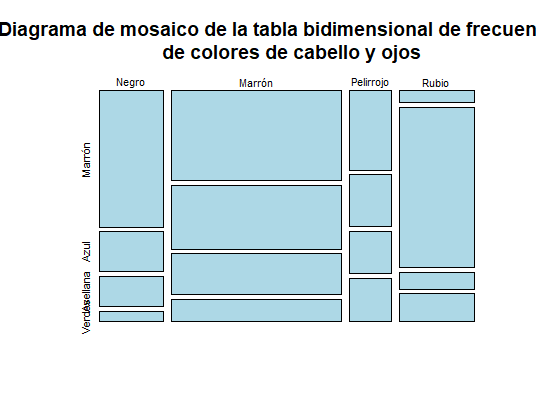
\includegraphics[scale=0.7]{Mosaico}
\caption{Representación grafica de mosaico}
\label{fig:Mosaico}
\end{figure}

\newpage


\subsection{Estadística descripitiva de una variable}

En las sigientes gáficas se muestra la variación que hay entre el color de cabello \ref{f:DensityCabello}, color de ojos   \ref{f:DensityOjos} y el género mayor volube en cuanto a distincion del color de ojos y cabello\ref{f:DensitySexo}, ya que estas son una variación. 
\newline
\newline
Esté tipo de gráficas visualiza la distribución de datos en un intervalo o período de tiempo continuo. Este gráfico es una variación de un Histograma que usa el suavizado de cerner para trazar valores, permitiendo distribuciones más suaves al suavizar el ruido. Los picos de un gráfico de densidad ayudan a mostrar dónde los valores se concentran en el intervalo.


\begin{figure}[h]
 \centering
  \subfloat[Cabello]{
   \label{f:DensityCabello}
    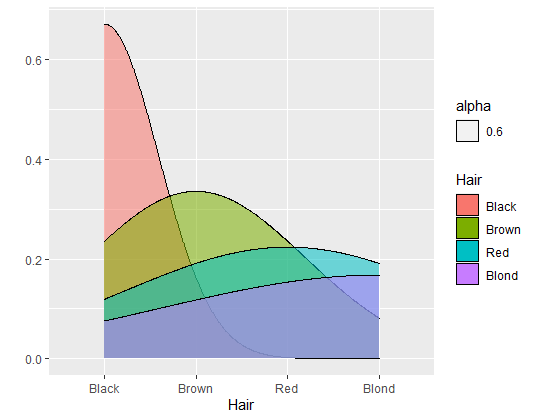
\includegraphics[width=0.3\textwidth]{DensityCabello}}
  \subfloat[Ojos]{
   \label{f:DensityOjos}
    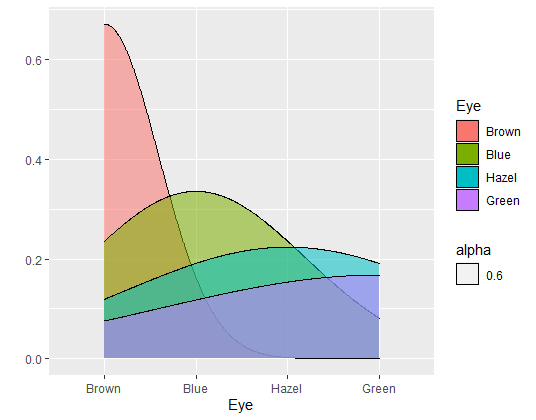
\includegraphics[width=0.3\textwidth]{DensityOjos}}
  \subfloat[Sexo]{
   \label{f:DensitySexo}
    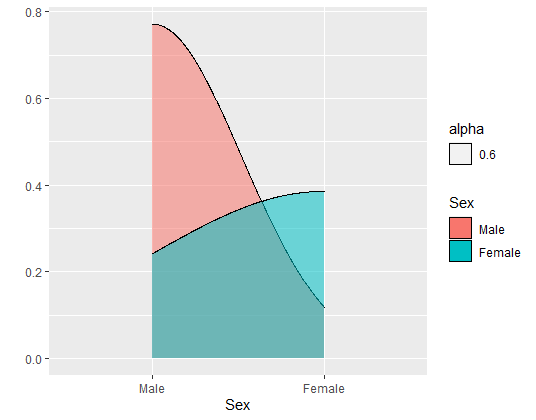
\includegraphics[width=0.3\textwidth]{DensitySexo}}
 \caption{Density plot de cabello, ojos y sexo}
 \label{f:Density}
\end{figure}

Su objetivo es extraer una tabla bidimensional de frecuencas absolutas de las variables Eye y hair, sin distinguir según el sexo. La manera más fácil de obtener esta tabla es sumando las subtabla de frecuencias para hombres y mujeres, y aplicando as.table() al resultado para transformarlo en una tabla por si no lo es.


\begin{table}[ht]
\centering
\label{f:FrecuenciaMinMax}
\begin{tabular}{|c|c|c|c|ll}
\cline{1-4}
\textbf{Hair}  & \textbf{Eye}  & \textbf{Sex}   & \textbf{Freq}          &  &  \\ \cline{1-4}
Black:8 & Brown:8 & Male:16   & Min.:2.00     &  &  \\ \cline{1-4}
Brown:8 & Blue :8 & Female:16 & 1st Qu.: 7.00 &  &  \\ \cline{1-4}
Red:8    & Hazel:8 &           & Median :10.00 &  &  \\ \cline{1-4}
Blond:8 & Green:8 &           & Mean:18.50    &  &  \\ \cline{1-4}
        &         &           & 3rd Qu.:29.25 &  &  \\ \cline{1-4}
        &         &           & Max.:66.00    &  &  \\ \cline{1-4}
\end{tabular}
   
 \caption{Frecuencia mediana, minima y maxima}
\label{f:FrecuenciaMedMinMax}
\end{table}

En la tabla se puede observar que la minima es de 2.00, una mediana de 10.00 y una maxima de 66.00, con el primer lugar de 7.00, segundo de 18.50 y tercero de 29.25.

De esto se desglosa  sus respectivas gráficas de frecuencia relativa entre la cantidad de color de ojos \ref{f:FrecuenciaOjos} y el color  de cabello  \ref{f:FrecuenciaCabello}.



\begin{figure}
 \centering
  \subfloat[Ojos]{
   \label{f:FrecuenciaOjos}
    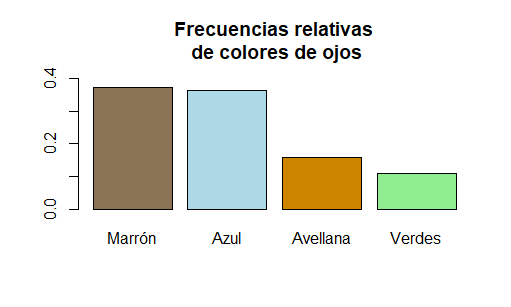
\includegraphics[width=0.4\textwidth]{FrecuenciaOjos}}
  \subfloat[Cabello]{
   \label{f:FrecuenciaCabello}
    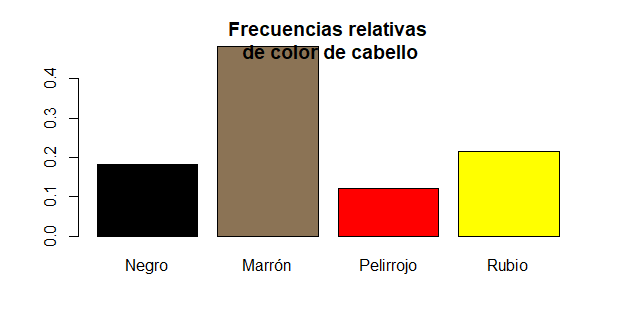
\includegraphics[width=0.4\textwidth]{FrecuenciaCabello}}
 \caption{Frecuencia de color de cabello y de ojos}
 \label{f:Frecuencias}
\end{figure}

\newpage


En comparacion a las gráficas anteriores, se muestran la correlatividad entre el color de cabello para cada color de ojos \ref{f:FrecuenciaOjosCabello} y las frecuencias relativas de colores de ojos para cada color de cabello \ref{f:FrecuenciaCabelloOjos}.


\begin{figure}[h]
 \centering
  \subfloat[Ojos]{
   \label{f:FrecuenciaOjosCabello}
    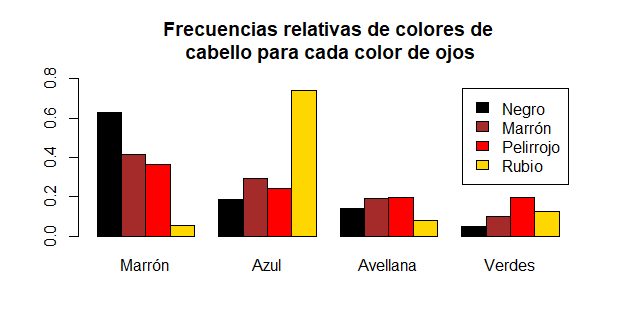
\includegraphics[width=0.4\textwidth]{FrecuenciaOjosCabello}}
  \subfloat[Cabello]{
   \label{f:FrecuenciaCabelloOjos}
    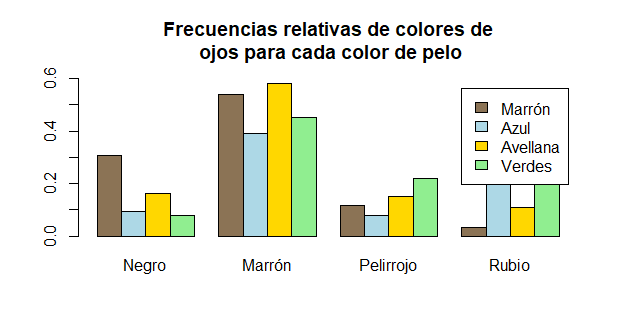
\includegraphics[width=0.4\textwidth]{FrecuenciaCabelloOjos}}
 \caption{Frecuencia correlativa entre el color de cabello y de ojos}
 \label{f:Frecuencias2}
\end{figure}

\newpage
\subsection{Estadística descripitiva de dos variable}


Boxplot de correlación \citep{RPubs}

El diagrama de caja es un gráfico utilizado para representar una variable cuantitativa (variable numérica). El gráfico es una herramienta que permite visualizar, a través de los cuartiles, cómo es la distribución, su grado de asimetría, los valores extremos, la posición de la mediana, etc.

En esté apartado se muestran tres Boxplot en relación a los datos Sexo \ref{f:Box1}, cabello \ref{f:BoxCabello} y ojos\ref{f:BoxOjos}


\begin{figure}[h]
 \centering
  \subfloat[Sexo]{
   \label{f:Box1}
    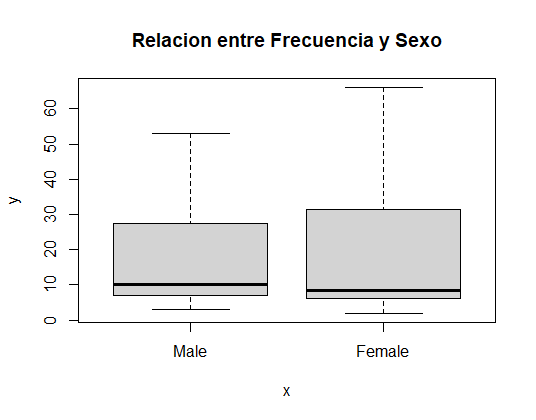
\includegraphics[width=0.3\textwidth]{Box1}}
  \subfloat[Cabello]{
   \label{f:BoxCabello}
    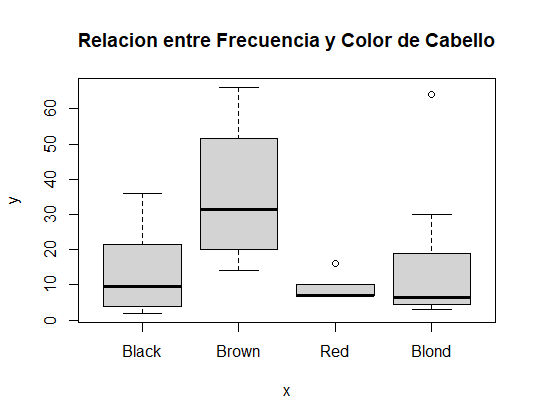
\includegraphics[width=0.3\textwidth]{BoxCabello}}
  \subfloat[Ojos]{
   \label{f:BoxOjos}
    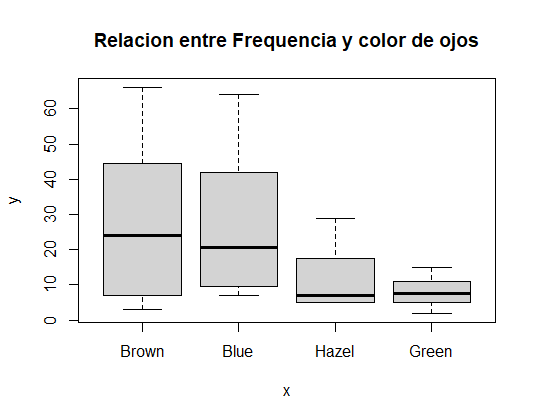
\includegraphics[width=0.3\textwidth]{BoxOjos}}
 \caption{Box de correlación entre frecuencia y las variables}
 \label{f:Box}
\end{figure}

De estos tres digramas de caja, se muestra que las mujeres tienen un mayor indice en comparacion a los hombre en cuanto al color del cabello y ojos, mientras que el color de cabello con mas indice es el cafe al igual que el color de los ojos.
\newline
\newline

A continuación se muestran otros dos diagramas que filtran esta informacion por género, en el cual el cabello cuenta con mayor indice de mujeres, las cuales tienen el cabello castaño, mientras que los hombres destacan con el color de ojos cafe y azul. 
Lo cual nos indica que el sexo masculino tiene un mayor indice de variación de iris \ref{f:BoxplotOjos} y las mujeres cuentan con mayor indice de cabello castaño \ref{f:BoxplotCabello}.

\begin{figure}[ht]
 \centering
  \subfloat[Cabello]{
   \label{f:BoxplotCabello}
    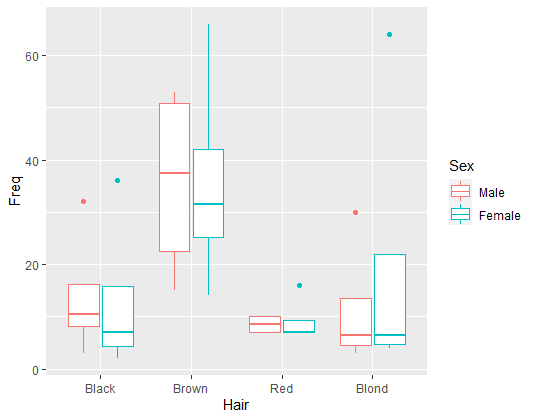
\includegraphics[width=0.4\textwidth]{BoxplotCabello}}
  \subfloat[Ojos]{
   \label{f:BoxplotOjos}
    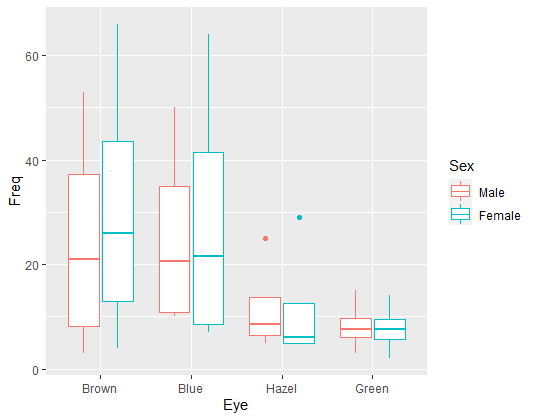
\includegraphics[width=0.4\textwidth]{BoxplotOjos}}
 \caption{Boxplot de correlación entre género y color de cabello y ojos}
 \label{f:Boxplot}
\end{figure}


\newpage
Escala [fig\ref{fig:Escala}] de variación entre género y frecuencia en el que se presentan los distintos colores de cabello junto con el color de ojos \citep{RChart}.

A continuación se desglosan dos tablas de las cuales se presenta su respectiva representación gráfica escalar; dichas tablas se dividen en 2, por el género masculino \ref{f:FMale} y género femenino \ref{f:FFemale}.

\begin{table}[h]
\centering
\label{Correlacion}
\begin{tabular}{|c|c|c|c|c|}
\hline
\textbf{Hair}  & \textbf{Eyes Brown} & \textbf{Eyes Blue} & \textbf{Eyes Hazel} & \textbf{Eyes Green} \\ \hline
\textbf{Black} & 32                  & 11                 & 10                  & 3                   \\ \hline
\textbf{Brown} & 53                  & 50                 & 25                  & 15                  \\ \hline
\textbf{Red}   & 10                  & 10                 & 7                   & 7                   \\ \hline
\textbf{Blond} & 3                   & 30                 & 5                   & 8                   \\ \hline
\end{tabular}
\caption{Tabla relativas entre cabello y ojos de género masculino}
\label{f:FMale}
\end{table}

\begin{table}[ht]
\centering
\label{Correlacion2}
\begin{tabular}{|c|c|c|c|c|}
\hline
\textbf{Hair}  & \textbf{Eyes Brown} & \textbf{Eyes Blue} & \textbf{Eyes Hazel} & \textbf{Eyes Green} \\ \hline
\textbf{Black} & 36                  & 9                  & 5                   & 2                   \\ \hline
\textbf{Brown} & 66                  & 34                 & 29                  & 14                  \\ \hline
\textbf{Red}   & 16                  & 7                  & 7                   & 7                   \\ \hline
\textbf{Blond} & 4                   & 64                 & 5                   & 8                   \\ \hline
\end{tabular}
\caption{Tabla relativas entre cabello y ojos de género femenino}
\label{f:FFemale}
\end{table}


\begin{figure}
\centering
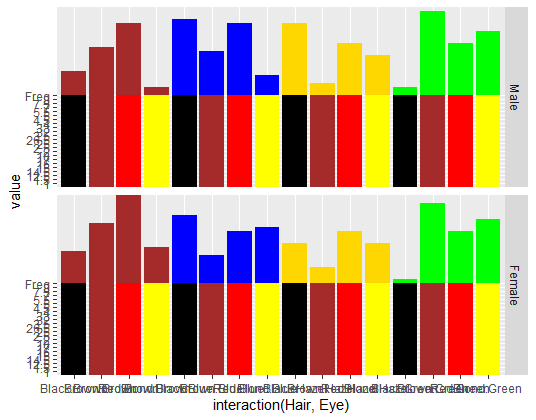
\includegraphics[scale=0.8]{Escala}
\caption{Escala de variación}
\label{fig:Escala}
\end{figure}

\newpage
\section{Conclusión}
La base de datos de HairEyesColor, se usa como referencia a las mediciones o frecuencia en que existe la relacion entre el color de cabello y ojos de las personas, llevando un listado de cada persona que fue medido y relacionado a este tipo. 

Los datos proporcionados por la base de datos fue de mucha ayuda ya que, al momento de buscar y realizar el filtramiento de la información para su representación gráfica, se tenia un mejor manejo de la informacion y su categorización por sexo.

Se mostraba un mejor manejo de datos, pero a la vez que esta era mas eficiente en su distribución, se teniene un menor rango para realizar un analísis mas profundo de diagramas.

Es interesante la investigación de datset en R, al igual que sus implicaciones en estadística, es manejable para numerosas cantidades de información de las cuales se puede tener un mayor indice de error y ser frustantes.

Se tuvo que realizar un exhaustivo procesamiento de códigos, ya que en si este tipo de base de datos se maneja mas por gráficas de mosaico y de indice, lo cual ocasionó que navegara en distintas fuentes y coementarios de usuarios en base a dudas o optimisación para la creación de escalas didacticas.\citep{repositorio}



\newpage

\section{Referencias}

\bibliography{biblio}
\bibliographystyle{plainnat}


\end{document}
